\documentclass[../Article_Model_Parameters.tex]{subfiles}
\graphicspath{{\subfix{../Figures/}}}
\begin{document}
		
	\subsubsection{Continuity equation} \label{CH: Continuity}
	 %When the cross-sectional area of the channel $A_f$ is specified as a function of the void fraction ${\color{black}\phi}(z)$ (where ${\color{black}\phi}$ is the void fraction of the bed and $A$ is the cross-section of the empty extractor), the continuity equation takes the form: %\todo[]{assign a color of v and u}
	 
	%The obtained above quasi-one-dimensional continuity equation (Equation \ref{EQ: CompressibleEuler_1}) is further modified by specifying a function ${\color{black}A_f}(z) = {\color{black}A\phi}(z)$ to take into account the change of the cross-section available for the fluid. The Equation \ref{EQ: Continuity_differential} shows the differential form of the continuity equation: 
	
	The previously derived quasi-one-dimensional continuity equation (Equation \ref{EQ: CompressibleEuler_1}) is refined by incorporating a function ${\color{black}A_f}(z) = {\color{black}A\phi}(z)$. This modification accounts for the variability in the cross-sectional area available for fluid flow. Equation \ref{EQ: Continuity_differential} presents this adaptation in the differential form of the continuity equation, capturing the dynamics of the flow as it responds to changes in the cross-section.
	
	{\footnotesize
		\begin{equation} \label{EQ: Continuity_differential}
			\frac{\partial ({\color{black}\rho_f}({\color{black}T}(t,z),{\color{black}P}(t)) {\color{black}\phi}(z))}{\partial t} + \frac{\partial ({\color{black}\rho_f}({\color{black}T}(t,z),{\color{black}P}(t)) v {\color{black}A\phi}(z))}{\partial {\color{black}z}} = 0
		\end{equation}
	}
	where ${\color{black} A}$ is the total cross-section of the extractor and ${\color{black}\phi}(z)$ describe porosity along the extractor.
	
	%{\color{black}assign a color of v and u}
	
	Assuming that the mass flow rate is constant in time, the temporal derivative becomes zero, and the spatial derivative can be integrated along ${\color{black}z}$ as
	
	{\footnotesize
		\begin{equation}
			\int \frac{\partial ({\color{black}\rho_f}({\color{black}T}(t,z),{\color{black}P}(t)) v {\color{black}A \phi}(z) )}{\partial {\color{black}z}} dz = 0 \rightarrow {\color{black}F}={\color{black}\rho_f}({\color{black}T}(t,z),{\color{black}P}(t)) v {\color{black}A\phi}(z)
		\end{equation}
	}
	
	Here, ${\color{black}F}$ is a constant obtained from the integration and is understood as the mass flux per unit area, which is assumed to be constant along ${\color{black}z}$. To simplify the dynamics of the system, it is assumed that ${\color{black}F}={\color{black}F}(t)$ is a control variable and affects the whole system instantaneously. This assumption allows for finding the velocity profile that satisfies mass continuity based on ${\color{black}F}(t)$, ${\color{black}\phi}(z)$, and ${\color{black}\rho_f}({\color{black}T}(t,z),{\color{black}P}(t))$.
	
	{\footnotesize
	\begin{equation}
		v = \cfrac{{\color{black}F}(t)}{{\color{black}\rho_f}({\color{black}T}(t,z),{\color{black}P}(t)) {\color{black}A\phi}(z)} 
	\end{equation}
	}
	
	The fluid density ${\color{black}\rho_f}({\color{black}T}(t,z),{\color{black}P}(t))$ can be obtained from an equation of state if temperature and the thermodynamic pressure (assumed ${\color{black}P}(t)$ to be constant along ${\color{black}z}$ due to the low-Mach number condition) are known. The variation in density may be caused by the fluid accumulation in the system (equivalent to pressure change), which occurs instantaneously along ${\color{black}z}$ or by a temperature change. 
	
	Analogously, the superficial velocity might be introduced to the model and defined as
	
	{\footnotesize
		\begin{equation}
			u = v {\color{black}\phi}(z) = \cfrac{{\color{black}F}(t)}{{\color{black}\rho_f}({\color{black}T}(t,z),{\color{black}P}(t)) {\color{black} A} }
		\end{equation}
	}
	
	\subsubsection{Mass balance for the fluid phase} \label{CH: Mass_balance_fluid}
	
	The comprehensive derivation of the mass balance equation for the fluid phase is detailed in Appendix \ref{CH: Gouverning equations}. This equation accounts for the movement of the pseudo-homogeneous fluid phase (Equation \ref{Model_fluid}), which is constrained to the axial direction due to the quasi-one-dimensional approach that considers changes in the void fraction. It is also predicated on the assumption that the thermodynamic pressure remains constant throughout the device, as illustrated by Equation \ref{EQ: Pressure_Velocity}. The analysis further simplifies the flow dynamics by disregarding the boundary layer near the extractor's inner wall, leading to a uniform velocity profile across any cross-section perpendicular to the axial direction. Given that the solute concentration in the solvent is negligible, the fluid phase is described as pseudo-homogeneous, with properties identical to the solvent itself. The mass balance equation thus encompasses convection, diffusion, and kinetic terms to accurately represent the fluid phase's behaviour.
	
	{\footnotesize
		\begin{equation}
			\label{Model_fluid}
			\frac{\partial {\color{black}c_f}(t,z)}{\partial t}
			+ \frac{1}{{\color{black}\phi}(z)} \frac{\partial \left( {\color{black}c_f}(t,z) u\right)}{\partial {\color{black}z}}
			= \frac{1-{\color{black}\phi}(z)}{{\color{black}\phi}(z)} {\color{black}r_e}(t,z)
			+ \frac{1}{{\color{black}\phi}(z)} \frac{\partial}{\partial {\color{black}z}} \left( {\color{black}D^M_e} \frac{\partial {\color{black}c_f}(t,z)}{\partial {\color{black}z}} \right)
		\end{equation}
	}
	
	${\color{black}c_f}(t,z)$ represents the concentration of solute in the fluid phase, , ${\color{black}r_e}(t,z)$ is a mass transfer kinetic term, and ${\color{black}D^M_e}({\color{black}T}(t,z),{\color{black}P}(t),{\color{black}F}(t))$ is the axial diffusion coefficient.
	
	\subsubsection{Mass balance for the solid phase} \label{Mass_balance_solid}
	
	The solid phase is considered to be stationary, without convection and diffusion terms in the mass balance equation (Equation \ref{Model_solid}). Therefore, the only significant term in this equation is the kinetic term (as defined in Equation \ref{Model_kinetic_basic}), which connects the solid and fluid phases. The extract is represented by a single pseudo-component to simplify the analysis. 
	
	{\footnotesize
		\begin{equation} 
			\label{Model_solid}
			%		{\scriptsize\begin{equation}
					\cfrac{\partial {\color{black}c_s}(t,z)}{\partial t} = \underbrace{ {\color{black}r_e}(t,z) }_{\text{Kinetics}}
			\end{equation} }
			
	\subsubsection{Kinetic term} \label{CH: Kinetic}
	
	%The kinetic term is based on two-film theory and follow work of \citet{Reverchon1996}. The mass transfer kinetic (Equation \ref{Model_kinetic_basic}) consists of the overall diffusion coefficient and the concentration gradient, which acts as a driving force for the process.
	
	The kinetic term in this study is based on the two-film theory proposed by \citet{Reverchon1996}, and the mass transfer kinetic is given by Equation \ref{Model_kinetic_basic}. This equation takes into account the overall diffusion coefficient and the concentration gradient, which acts as the driving force for the process.
	
%	As the solvent flows through the bed, the $CO_2$ molecules diffuse into the pores and adsorb on the particle surface to form an external fluid film around the solid particles through the solvent–solid matrix interactions. Assuming that the mean free path of the molecule is much smaller than the pore diameter, the effect of Knudsen diffusion is small and can be neglected. The dissolved solute diffuses from the particle's core through the solid-fluid interface, the pore, and the film into the bulk. The graphical representation of the mass transfer mechanism is shown in Figure \ref{fig: SFE_Mechanism}. The mean solute concentration in the solid phase is denoted as ${\color{black}c_s}$. At the solid-fluid interface, the equilibrium concentrations are given as ${\color{black}c_s^*}$ and ${\color{black}c_P^*}$, respectively for solid and fluid phases. The concentration of the solutes in the fluid phase in the centre of the pore is denoted as ${\color{black}c_{P}}$. As the solute diffuses through the pore, its concentration changes and reaches ${\color{black}c_{Pf}}$ at the opening of the pore. The solute diffuses through the film around the particle and reaches a concentration in the bulk ${\color{black}c_f}$. It can be assumed that the two-film theory describes the solid-fluid interface inside the pore. The overall mass transfer coefficient can be introduced if the relation between the solute concentration in one phase and its equilibrium concentration is known.
	
	As the solvent flows through the bed, $CO_2$ molecules diffuse into the pores and adsorb on the particle surface to form an external fluid film around the solid particles due to the solvent-solid matrix interactions. The effect of Knudsen diffusion is negligible in this process, as the mean free path of the molecule is much smaller than the pore diameter. The dissolved solute diffuses from the particle's core through the solid-fluid interface, the pore, and the film into the bulk. Figure \ref{fig: SFE_Mechanism} illustrates the mass transfer mechanism, where the mean solute concentration in the solid phase is denoted as ${\color{black}c_s}$ and the equilibrium concentrations at the solid-fluid interface are denoted as ${\color{black}c_s^*}$ and ${\color{black}c_p^*}$, respectively, for solid and fluid phases. The concentration of the solutes in the fluid phase in the center of the pore is denoted as ${\color{black}c_{p}}$. As the solute diffuses through the pore, its concentration changes and reaches ${\color{black}c_{pf}}$ at the opening of the pore. The solute then diffuses through the film around the particle and reaches bulk concentration ${\color{black}c_f}$. The two-film theory describes the solid-fluid interface inside the pore. The overall mass transfer coefficient can be determined if the relationship between the solute concentration in one phase and its equilibrium concentration is known.
			
		\begin{figure}[h!]
			\centering
			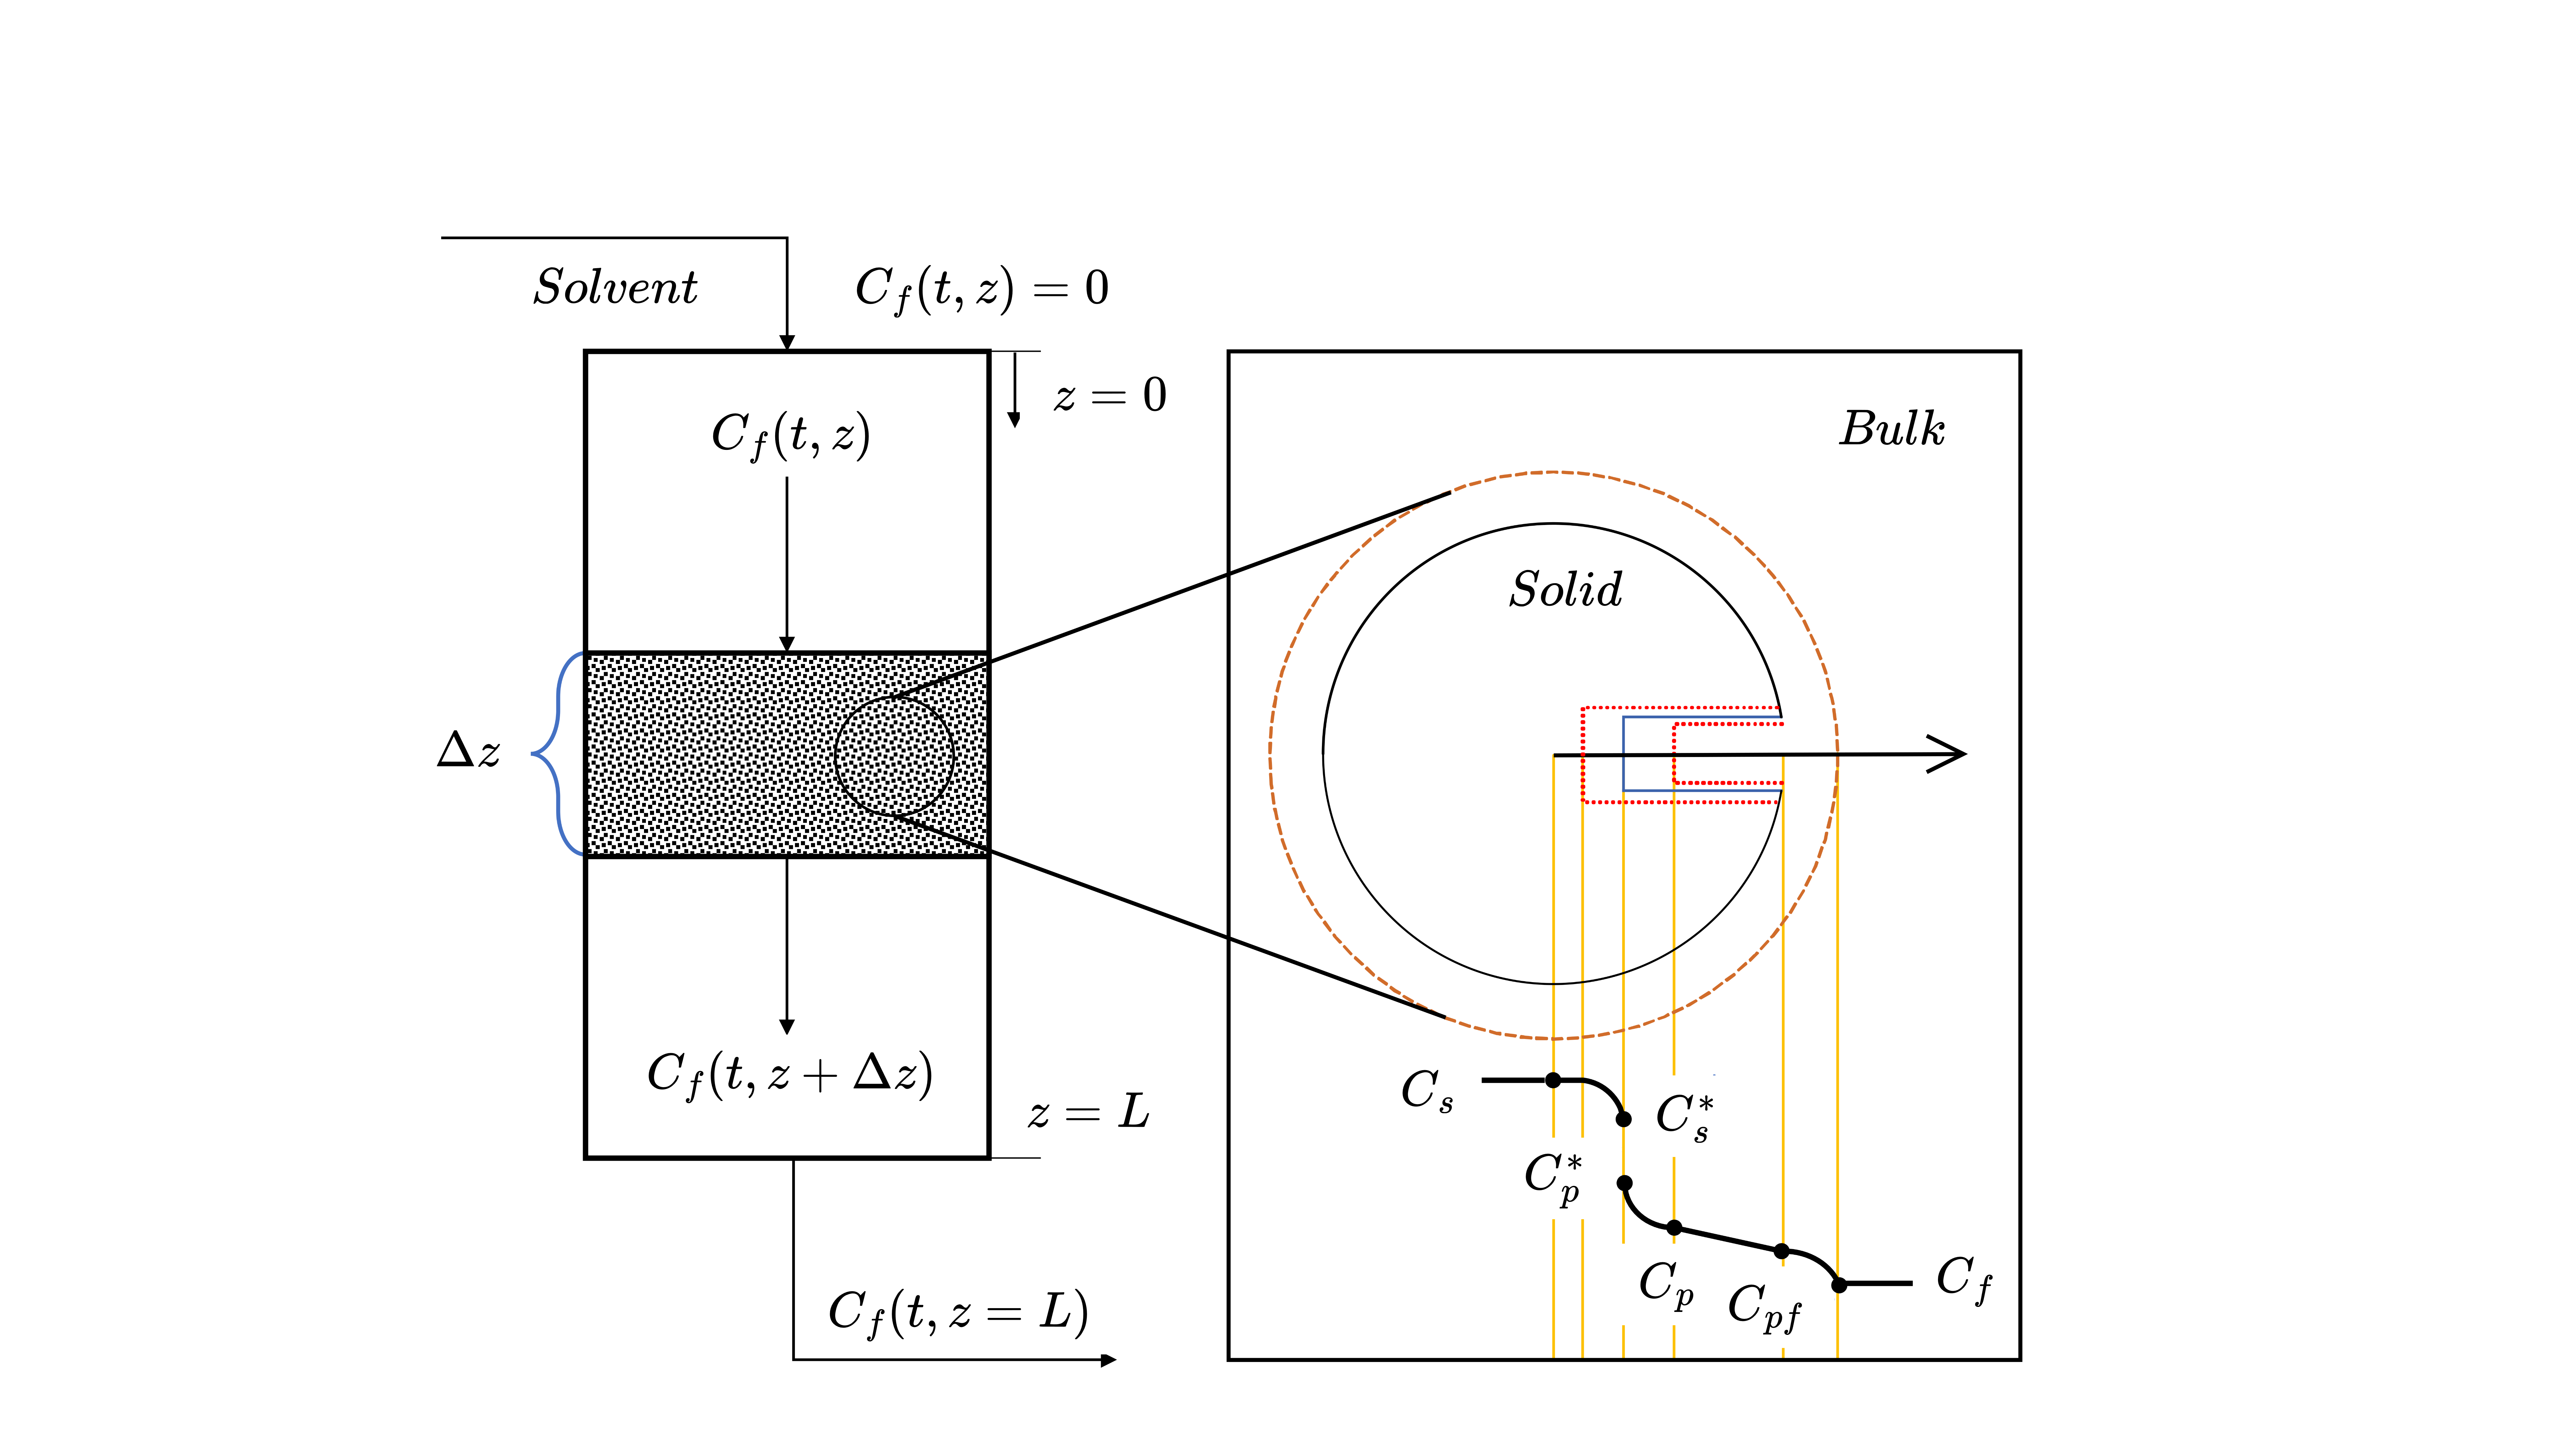
\includegraphics[trim = 45cm 0cm 60cm 20cm,clip,width=\columnwidth]{Figures/SFE_PFD.drawio.png}	
			\caption{The extraction mechanism}
			\label{fig: SFE_Mechanism}
		\end{figure}
			
		\citet{Bulley1984} suggests a process where the driving force for extraction is given by the difference between the concentration of the solute in bulk, ${\color{black}c_f}$, and in the center of the pore, ${\color{black}c_p^*}$. The concentration ${\color{black}c_p^*}$ is in equilibrium with ${\color{black}c_s}$ according to an equilibrium relationship. The rate of extraction is thus ${\color{black}r_\text{e}}\left({\color{black}c_f} - {\color{black}c^*_p}({\color{black}c_s})\right)$.  
			
		On the other hand, \citet{Reverchon1996} proposes a driving force given by the difference between ${\color{black}c_s}$ and ${\color{black}c_p^*}$. ${\color{black}c_p^*}$ is determined by an equilibrium relationship with ${\color{black}c_f}$ and the extraction rate is ${\color{black}r_\text{e}}\left({\color{black}c_s} - {\color{black}c^*_p}({\color{black}c_f})\right)$ or more precisely
			
			{\footnotesize
				\begin{equation} \label{Model_kinetic_basic}
					{\color{black}r_e}(t,z) = \cfrac{{\color{black}D_i}({\color{black}T}(t,z), {\color{black}P}(t), F(t))}{{\color{black} \mu l^2} }\left({\color{black}c_s}(t,z) - {\color{black}c_P^*}(t,z) \right)
			\end{equation} }
			
		where ${\color{black}\mu}$ is sphericity, ${\color{black}l}$ a characteristic dimension of particles and can be defined as ${\color{black}l} = {\color{black}r}/3$, ${\color{black}r}$ is the mean particle radius, ${\color{black}\rho_s}$ is the solid density, ${\color{black}D_i}({\color{black}T}(t,z))$ corresponds to the overall diffusion coefficient and ${\color{black}c_P^*}(t,z)$ is a concentration at the solid-fluid interface (which according to the internal resistance model is supposed to be at equilibrium with the fluid phase). 
			
		According to \citet{Bulley1984}, a linear equilibrium relationship (equation  \ref{Linear_equilibirum}) can be used to find an equilibrium concentration of the solute in the fluid phase ${\color{black}c_f^*}(t,z)$ is based on the concentration of the solute in the solid phase ${\color{black}c_s}(t,z)$ 
			
			{\footnotesize
				\begin{align} \label{Linear_equilibirum}
					{\color{black}c}(t,z) &= {\color{black}k_p}({\color{black}T}(t,z),{\color{black}P}(t)) \allowbreak {\color{black}q^*}(t,z)
			\end{align} }
			
			The volumetric partition coefficient ${\color{black}k_p}({\color{black}T}(t,z),{\color{black}P}(t))$ behaves as an equilibrium constant between the solute concentration in one phase and the corresponding equilibrium concentration at the solid-fluid interphase. According to \citet{Spiro2007}, the term ${\color{black}k_p}({\color{black}T}(t,z),{\color{black}P}(t))$ can be expressed as the function of mass partition factor ${\color{black}k_m}({\color{black}T}(t,z))$.
			
			{\footnotesize
				\begin{align}
					{\color{black}k_m}({\color{black}T}(t,z)) = \cfrac{{\color{black}k_p}({\color{black}T}(t,z),{\color{black}P}(t)) {\color{black}\rho_s}}{{\color{black}\rho}({\color{black}T}(t,z),{\color{black}P}(t))}
			\end{align} }
			
			Equation \ref{Model_kinetic_no_sat} represents of the kinetic term according to \citet{Reverchon1996}
			
			{\footnotesize
				\begin{equation}
					\label{Model_kinetic_no_sat}
					{\color{black}r_e}(t,z) = -\cfrac{{\color{black}D_i}({\color{black}T}(t,z), {\color{black}P}(t), F(t))}{{\color{black} \mu l^2} }\left({\color{black}c_s}(t,z) - \cfrac{{\color{black}\rho_s}c_f(t,z)}{{\color{black}k_m}({\color{black}T}(t,z)){\color{black}\rho_f}({\color{black}T}(t,z),{\color{black}P}(t))}   \right)
			\end{equation} }

        \subfile{Saturation}
		
		\iffalse	
		\subsubsection{Heat balance} \label{CH: heat_balance}
		
		 {\color{black}
			The heat balance (Equation \ref{Model_heat}) consists of the convective and diffusive terms. It follows the assumption of a pseudo-homogeneous phase, which properties are the mean between fluid and solid phases. We consider no heat loss through the wall, and there is no heat generation in the system. Therefore, the temperature of the extractor can be changed only by manipulating the temperature of the inlet stream %$T_{In}(t)$. 
			
			We assume that at a given section, where the cross-sectional area is $A$, the flow properties are uniform across that section. Hence, although the area of an extractor changes  as a function of a distance along an extractor (e.g. if a fixed fill an extractor partially), $z$, and therefore in reality the flow field is two-dimensional (the flow varies in the two-dimensional space), we make the assumption that the flow properties vary only with $z$; this is tantamount to assuming uniform properties across any given cross section. Such flow is defined as quasi-one-dimensional flow.
			
		}
		
		\sout{The heat balance equation (equation  \ref{Model_heat}) was developed, assuming the existence of a pseudo-homogeneous phase, which properties are the mean between fluid and solid phases (the amount of solute is considered small enough not to affect the overall heat balance). Equation \ref{Model_heat} contains the convection and the diffusion terms. It is considered that there is no heat loss through the wall, and there is no heat generation in the system. The temperature of the extractor can be changed only by increasing the temperature of the inlet stream. The pseudo-homogenous phase is assumed to flow only in the axial direction. The numerator of the factor in front of the convection term of the heat equation contains only the specific heat of the fluid ${\color{black}C_p}({\color{black}T}(t,z),{\color{black}P}(t))$ because the solid phase is stationary. Therefore, this factor can be understood as the fraction of the fluid's total heat through convection. On the other hand, the axial heat diffusion is calculated based on the definition of thermal diffusivity for the fluid, as explained in Appendix. }
			
		{\color{black} The heat balance (Equation \ref{Model_heat}), is based on \citet{Srinivasan2012}, and consists of convective and diffusive terms. It follows the assumption of a pseudo-homogeneous phase, which properties are the mean between fluid and solid phases. It is considered that there is no heat loss through the walls, and there is no heat generation in the system. The temperature of the extractor can be changed only by manipulating the temperature of the inlet stream ${\color{black}T_{Inlet}}(t)$.
			}
			
			{\footnotesize
				\begin{equation} \label{Model_heat}
					\begin{split}
						\cfrac{\partial {\color{black}T}(t,z)}{\partial t} &= 
						\underbrace{ -\cfrac{{\color{black}F}(t) {\color{black}C_p}({\color{black}T}(t,z),{\color{black}P}(t))}{{\color{black}A} 	[(1-{\color{black}\epsilon}){\color{black}\rho_f}({\color{black}T}(t,z),{\color{black}P}(t)) {\color{black}C_p} ({\color{black}T}(t,z),{\color{black}P}(t)) + {\color{black} \epsilon \rho_s C_{ps} } ]} \cfrac{\partial {\color{black}T}(t,z)}{\partial {\color{black}z}}  }_{\text{Convection}} + \\
						& + \underbrace{ {\color{black}D^T_e}({\color{black}T}(t,z),{\color{black}P}(t)) \cfrac{\partial^2 {\color{black}T}(t,z)}{\partial {\color{black}z^2}} }_{\text{Diffusion}}
					\end{split}
			\end{equation} }
			
		where $ {\color{black}D^M_e}({\color{black}T}(t,z),{\color{black}P}(t),{\color{black}F}(t))$ is the axial mass diffusion coefficient, ${\color{black}C_p}({\color{black}T}(t,z),{\color{black}P}(t))$ is the fluid's specific heat, ${\color{black}C_{ps}}$ is the specific heat of the solid phase, ${\color{black}D^T_e}({\color{black}T}(t,z),{\color{black}P}(t),{\color{black}F}(t))$ is the axial heat diffusion coefficient. 

%		\todo[inline]{Draft of new heat equation starts here. TODO: \\ Check if the heat cpacity of solid phase needs to be added \\ Elaborate why pressure is know}
		
			The heat governing equation describe the evolution of the energy in the system and it is given by \ref{EQ: Heat_internal}. The derivation of the heat equation can be found in Appendix \ref{CH: Gouverning equations}.
			
			{\footnotesize
			\begin{align} \label{EQ: Heat_internal}
				&\cfrac{\partial \left( {\color{black}\rho_f}({\color{black}T}(t,z),{\color{black}P}(t)) {\color{black}e}(t,z) A_f \right) }{\partial t} + \cfrac{\partial \left( {\color{black}\rho_f}({\color{black}T}(t,z),{\color{black}P}(t)) A_f v {\color{black}e}(t,z) \right)}{\partial {\color{black}z}} \nonumber \\
				&= -{\color{black}P}(t)\cfrac{\left( A_f v \right)}{\partial {\color{black}z}} + \cfrac{\partial}{\partial {\color{black}z}} \left( \cfrac{\partial {\color{black}T}(t,z)}{\partial {\color{black}z}} \right) 
			\end{align}
			}
		
			The departure function is a mathematical function that characterizes the deviation of a thermodynamic property (enthalpy, entropy, and internal energy) of a real substance from that of an ideal gas at the same temperature and pressure. The departure function is typically defined as the difference between the value of a thermodynamic property for a real fluid and the corresponding value for an ideal gas at the same temperature and pressure. They are typically computed by integrating a function that depends on the equation of state and its derivatives. Following \citet{Elliott2011} or \citet{Gmehling2019}, a real gas internal energy definition can be obtained from the departure functions, defined through Equation \ref{EQ: internal_energy_def}. More information on the departure functions can be found in Appendix \ref{CH:Enthalpy}.

			{\footnotesize
				\begin{equation}
					d{\color{black}e}(t,z)=C_vd{\color{black}T}-\left[{\color{black}P}(t)-{\color{black}T}(t,z)\left(\cfrac{\partial {\color{black}P}(t)}{\partial {\color{black}T}(t,z)}\right)_{{\color{black}v_m}\left({\color{black}T}(t,z), {\color{black}P}(t)\right)}\right]d{\color{black}v_m}\left({\color{black}T}(t,z), {\color{black}P}(t)\right)
					\label{EQ: internal_energy_def}
				\end{equation} }
			
			where ${\color{black}e}^{id}(t,z)$ is the internal energy of perfect gas.
			
			Suppose a gas is considered to be perfectly caloric (${\color{black}e}(t,z)={\color{black}C_v} {\color{black}T}(t,z)$), then the energy equation can be written explicitly in the form of temperature. The perfectly caloric gas can be seen as the special case of a real gas, where the second term of Equation \ref{EQ: internal_energy_def} goes to zero and the heat capacity ${\color{black}C_v}$ is constant.
			
			For real gases, it is complicated to write the heat balance in terms of temperature, but it can be used directly in the form of internal energy, as it is given by Equation \ref{EQ: CompressibleEuler_3}. In such a case, the temperature needs to be recovered from the internal energy. A relation for the internal energy can be obtained from an equation of state. For Peng-Robinson, such a relation is given by Equation \ref{EQ: internal_energy_PR} as presented by \citet{Elliott2011}.
			
%			{\footnotesize
%				\begin{equation}
%					e = C_vT + \cfrac{a\left(\alpha -T\cfrac{d \alpha}{dT}\right)}{2\sqrt{2}b} \ln \left[ \cfrac{1+b\left(1-\sqrt{2}\rho\right) }{1+b\left(1+\sqrt{2}\rho\right)} \right]
%					\label{EQ: internal_energy_PR}
%				\end{equation}
%			}
		
			{\scriptsize
				\begin{equation}
					\begin{aligned}
					&\cfrac{{\color{black}e}(t,z)-{\color{black}e}^{id}(t,z)}{R{\color{black}T}(t,z)} = \\
					& - \cfrac{{\color{black}A}\left({\color{black}T}(t,z), {\color{black}P}(t)\right)}{{\color{black}B}\left({\color{black}T}(t,z), {\color{black}P}(t)\right)\sqrt{8}} \cfrac{{\color{black}\kappa} \sqrt{\color{black}T_r}}{\sqrt{\alpha}} \ln \left[ \cfrac{{\color{black}Z}\left({\color{black}T}(t,z), {\color{black}P}(t)\right)+\left( 1+\sqrt{2} \right){\color{black}B}\left({\color{black}T}(t,z), {\color{black}P}(t)\right)}{{\color{black}Z}\left({\color{black}T}(t,z), {\color{black}P}(t)\right)+\left( 1-\sqrt{2} \right){\color{black}B}\left({\color{black}T}(t,z), {\color{black}P}(t)\right)} \right]
					\label{EQ: internal_energy_PR}
				\end{aligned}
			\end{equation}
			}
			
			To solve Equation \ref{EQ: internal_energy_PR}, temperature, pressure, and density values need to be known. If an equation of state is introduced, then only two out of three variables need to be obtained as the third one can be calculated; this can be represented as follow
			
			{\footnotesize
			\begin{equation}
				{\color{black}e}(t,z)={\color{black}e}({\color{black}T}(t,z),{\color{black}P}(t),{\color{black}\rho_f}({\color{black}T}(t,z),{\color{black}P}(t)))=e( {\color{black}T}(t,z),{\color{black}P}(t), {\color{black}\rho_f}({\color{black}T}(t,z),{\color{black}P}(t)) ) 
			\end{equation}
			}
		
			If the value of internal energy ${\color{black}e}(t,z)$ is known from the time evolution of the energy Equation \ref{EQ: CompressibleEuler_3}, and pressure is known from measurement, then the temperature can be reconstructed. A roootfinder can be used to find a value of temperature, which minimizes the difference between the value of internal energy coming from the time evolution (Equation \ref{EQ: Heat_internal}) and the output from Equation \ref{EQ: internal_energy_PR}. Such a procedure allows to find a local temperature along spatial direction ${\color{black}z}$ and needs to be repeated every time-step.
		
			Another way to express the energy equation is to introduce enthalpy ${\color{black}h}(t,z) = {\color{black}e}(t,z) + {\color{black}P}(t) / {\color{black}\rho_f}({\color{black}T}(t,z),{\color{black}P}(t))$. By introducing the definition of enthalpy, the energy equation becomes
			
			{\footnotesize
				\begin{align} \label{EQ:Enthalpy_equation}
					\cfrac{\partial \left({\color{black}\rho_f}({\color{black}T}(t,z),{\color{black}P}(t)) {\color{black}h}(t,z) A_f\right)}{\partial t} &= - \cfrac{\partial \left( {\color{black}\rho_f}({\color{black}T}(t,z),{\color{black}P}(t)) {\color{black}h}(t,z) A_f v \right)}{\partial {\color{black}z}}  \nonumber \\
					& + \cfrac{\partial \left({\color{black}P}(t) A_f\right)}{\partial t} + \cfrac{\partial}{\partial {\color{black}z}} \left( k \cfrac{\partial {\color{black}T}(t,z)}{\partial {\color{black}z}} \right)
				\end{align}
			}
		
			The main advantage of this formulation is the presence of term $\partial {\color{black}P}(t) / \partial t $, which allows it to directly affect the system through the change of thermodynamic pressure (which is a control variable). The enthalpy is related to the pressure and temperature through the following equation:
			
			{\footnotesize
				\begin{equation}
					{\color{black}h}(t,z)={\color{black}h}({\color{black}T}(t,z),{\color{black}P}(t),{\color{black}\rho_f}({\color{black}T}(t,z),{\color{black}P}(t)))={\color{black}h}( {\color{black}T}(t,z),{\color{black}P}(t), {\color{black}\rho_f}({\color{black}T}(t,z),{\color{black}P}(t)) ) 
					\label{EQ:Enthalpy_root}
				\end{equation}
			}
		
			If the value of enthalpy is known from the time evolution and pressure can be measured, then the Equation \ref{EQ:Enthalpy_root} can be solved for the temperature to recover the temperature profile. For the Peng-Robinson EoS, the enthalpy can be defined by Equation \ref{EQ:Enthalpy_PR}. More details can be found in Appendix \ref{CH:Enthalpy} or given by \citet{Gmehling2019}.
			
			{\scriptsize
				\begin{equation}
					\begin{split}
					{\color{black}h}(t,z)-{\color{black}h}(t,z)^{id}={\color{black}R}{\color{black}T}(t,z) \left[{\color{black}T_r}({\color{black}Z}\left({\color{black}T}(t,z), {\color{black}P}(t)\right)-1) \right. \\
					\left. -2.078(1+{\color{black}\kappa} ){\sqrt { {\color{black}\alpha}\left({\color{black}T}(t,z)\right) } } \ln \left(\cfrac{{\color{black}Z}\left({\color{black}T}(t,z), {\color{black}P}(t)\right)+\left( 1+\sqrt{2} \right){\color{black}B}\left({\color{black}T}(t,z), {\color{black}P}(t)\right)}{{\color{black}Z}\left({\color{black}T}(t,z), {\color{black}P}(t)\right)+\left( 1-\sqrt{2} \right){\color{black}B}\left({\color{black}T}(t,z), {\color{black}P}(t)\right)}\right)\right]
					\label{EQ:Enthalpy_PR}
				\end{split}
			\end{equation}				
			}
		
			The Equation \ref{EQ:Enthalpy_PR} requires an reference sate, which in this case is assumed to be ${\color{black}T_{ref}}=298.15~[K]$ and ${\color{black}P_{ref}}=1.01325~[bar]$.
			
			As discussed by \citet{Gmehling2019}, the influence of the intermolecular forces on the enthalpy is needs to taken into account in high pressures systems. In most cases, these forces are attractive, so additional energy is necessary to move the molecules away from each other, that is, to lower the density. If this energy is not added, the substance cools down when it is expanded.
			
		\subsubsection{Pressure term} \label{CH: Pressure}
		
		The pressure term in the energy equation, given by Equation \ref{EQ:Enthalpy_equation}, describes the change of the thermodynamic pressure with respect to time. As explained in Chapters \ref{CH:Governing_equations_chapter}, at Low-Mach number conditions, the thermodynamic pressure is nearly constant in space due to the small pressure wave propagation that occurs at the speed of sound. Under such conditions, the term $\partial {\color{black}P}/\partial t$ can be approximated by an ordinary differential equation, which describes the instantaneous change of pressure in the system. The pressure (P) in the system is considered a state variable, while the pressure in the new time-step ($P_{in}$) is considered a control variable.
		
		{\footnotesize
			\begin{equation}
				\frac{\partial {\color{black}P}(t)}{\partial t} \approx \frac{{\color{black}P}(t) - {\color{black}P_{in}}(t) }{\Delta t}
		\end{equation}}
		
		Such a simplified equation takes into account the pressure change in the energy balance, but the dynamics are simplified and do not consider the effects of pressure losses. In a real system, the dynamics of pressure change would depend on a pump used in an extraction system, as well as a back-pressure regulator used to control an outlet valve.
  		
  		\fi
  		
		\subsubsection{Extraction yield} \label{CH: Yield}
			
		The efficiency of the process (the yield) is calculated according to Equation \ref{Model_measurment_1} as presented by \citet{Sovova1994a}. The measurement equation evaluate the mass of solute at the outlet of the extraction unit and sums it. The integral form of the measurement equation (\ref{Model_measurment_1}) can be transformed into the differential form (\ref{Model_measurment_2}) and augmented with the process model.
			
		{\footnotesize
			\begin{align} 
				\label{Model_measurment_1}
%				y(t) \left[ kg \right] &= \int_{t_0}^{t_f} Q(t,z) \left[ \cfrac{m^3}{s} \right] c_f(t,z) \biggr\rvert_{z=L} \left[ \cfrac{kg}{m^3} \right] dt \left[ s \right] \\
				{\color{black}y}(t) &= \int_{t_0}^{t_f} \cfrac{{\color{black}F}(t)}{{\color{black}\rho_f}({\color{black}T}(t,z),{\color{black}P}(t))} {\color{black}c_f}(t,z) \biggr\rvert_{z=L} dt \\
%				\cfrac{dy}{dt} \left[ \cfrac{kg}{s} \right] &= Q(t,z) \left[ \cfrac{m^3}{s} \right] c_f(t,z) \biggr\rvert_{z=L} \left[ \cfrac{kg}{m^3} \right]  \\
				\cfrac{d{\color{black}y}(t)}{dt} &= \qquad \cfrac{{\color{black}F}(t)}{{\color{black}\rho_f}({\color{black}T}(t,z),{\color{black}P}(t))} {\color{black}c_f}(t,z) \biggr\rvert_{z=L} 
                \label{Model_measurment_2}
		\end{align}	}
  
		\subsubsection{Initial and boundary conditions} 
		It is assumed that the solvent is free of solute at the entrance of the extractor and that all the solid particles have the same initial solute content ${\color{black}c_{s0}}$. As the residence time is much shorter than the sampling time, the initial state estimate for the concentration of the solute in the fluid phase would be not reliable. Considering that it is assumed that the $c_{f0}=0$. Moreover, it is considered that the extractor is isothermal %and described by ${\color{black}h_0}$. 
		Therefore, the initial and boundary conditions employed in the simulation are:
			
		\begin{comment}
		{\footnotesize
				\begin{align*}
					&{\color{black}c_f}(t = 0, z) = 0 & {\color{black}c_s}(t = 0, z) = {\color{black}c_{s0}} & &{\color{black}h}(t = 0, z) = {\color{black}h_0} \\
					&\frac{\partial c_f(t,z=L)}{\partial x} = 0 & {\color{black}c_s}(t = 0, z) = {\color{black}c_{s0}} & &\frac{\partial h(t,z=L)}{\partial x} = 0
				\end{align*} }
		\end{comment}
			
			{\footnotesize
				\begin{align*}
					&{\color{black}c_f}(t = 0, z) = 0 & {\color{black}c_s}(t = 0, z) = {\color{black}c_{s0}} &{c_f}(t, z=0) = 0 \\
					&\frac{\partial c_f(t,z=0,L)}{\partial x} = 0 & c_s(t, z=0,L) = {\color{black}c_{s0}} &y(0) = 0
			\end{align*} }
			
		\subsubsection{Discretization methods}
		
		The method of lines is used to transform the process model equations into a set of ODEs denoted as ${\color{black}G}({\color{black}x}(t);{\color{black}\Theta})$. The partial derivatives in $z$-direction are computed using a first-order and second-order finite difference approximation. The backward finite difference is used to approximate the first-order derivative, while the central difference scheme is used to approximate the second-order derivative. The length of the fixed bed is divided into $N_z$ equally distributed points in $z$-direction. The state-space model after the discretization is represented by $\dot{{\color{black}x}}(t)$.
		
		\begin{comment}
		{\footnotesize
			\begin{align*} \label{discretization}
				\dot{{\color{black}x}}(t) &= \cfrac{d {\color{black}x}(t)}{d t} = 
				\begin{bmatrix}
					\cfrac{d {\color{black}c_{f,1}}(t)}{d t} 	  \\
					\vdots					  \\
					\cfrac{d {\color{black}c_{f,N_z}}(t)}{d t} \\
					\\ \hline \\
					\cfrac{d {\color{black}c_{s,1}}(t)}{d t} 	  \\
					\vdots					  \\
					\cfrac{d {\color{black}c_{s,N_z}}(t)}{d t} \\
					\\ \hline \\
					\cfrac{d {\color{black}h_1}(t)}{d t} 	  \\
					\vdots 					  \\
					\cfrac{d {\color{black}h_{N_z}}(t)}{d t} \\
					\\ \hline \\
					\cfrac{d {\color{black}P}(t)}{d t} \\
					\\ \hline \\
					\cfrac{d {\color{black}y}(t)}{d t}
				\end{bmatrix}
				=
				\underbrace{\begin{bmatrix}
						{\color{black}G_1} \left( {\color{black}c_f}(t),{\color{black}c_s}(t),{\color{black}h}(t); {\color{black}\Theta} \right)\\ 
						\vdots\\ 
						{\color{black}G_{N_z}} \left( {\color{black}c_f}(t),{\color{black}c_s}(t),{\color{black}h}(t); {\color{black}\Theta} \right)\\ 
						\\ \hline \\ \\
						{\color{black}G_{N_z+1}} \left( {\color{black}c_f}(t),{\color{black}c_s}(t),{\color{black}h}(t); {\color{black}\Theta} \right)\\ 
						\vdots\\
						{\color{black}G_{2N_z}} \left( {\color{black}c}(t),{\color{black}c_s}(t),{\color{black}h}(t); {\color{black}\Theta} \right)\\ 
						\\ \\ \hline \\ 
						{\color{black}G_{2N_z+1}} \left( {\color{black}c_f}(t),{\color{black}c_s}(t),{\color{black}h}(t); {\color{black}\Theta} \right) \\
						\vdots\\
						{\color{black}G_{3N_z}} \left( {\color{black}c_f}(t),{\color{black}c_s}(t),{\color{black}h}(t); {\color{black}\Theta} \right) \\ 
						\\ \\ \hline \\
						{\color{black}G_{3N_z+1}} \left( {\color{black}c_f}(t),{\color{black}c_s}(t),{\color{black}h}(t); {\color{black}\Theta} \right) \\
						\\ \\ \hline \\
						{\color{black}G_{3N_z+2}} \left( {\color{black}c_f}(t),{\color{black}c_s}(t),{\color{black}h}(t); {\color{black}\Theta} \right) 
				\end{bmatrix}}_{{\color{black}G} \left( {\color{black}x}(t); {\color{black}\Theta} \right)} 
		\end{align*} }
	\end{comment}
		
		{\footnotesize
			\begin{align*} \label{discretization}
				\dot{{\color{black}x}}(t) &= \cfrac{d {\color{black}x}(t)}{d t} = 
				\begin{bmatrix}
					\cfrac{d {\color{black}c_{f,1}}(t)}{d t} 	  \\
					\vdots					  \\
					\cfrac{d {\color{black}c_{f,N_z}}(t)}{d t} \\
					\\ \hline \\
					\cfrac{d {\color{black}c_{s,1}}(t)}{d t} 	  \\
					\vdots					  \\
					\cfrac{d {\color{black}c_{s,N_z}}(t)}{d t} \\
					%\\ \hline \\
					%\cfrac{d {\color{black}P}(t)}{d t} \\
					\\ \hline \\
					\cfrac{d {\color{black}y}(t)}{d t}
				\end{bmatrix}
				=
				\underbrace{\begin{bmatrix}
						{\color{black}G_1} \left( {\color{black}c_f}(t),{\color{black}c_s}(t); {\color{black}\Theta} \right)\\ 
						\vdots\\ 
						{\color{black}G_{N_z}} \left( {\color{black}c_f}(t),{\color{black}c_s}(t); {\color{black}\Theta} \right)\\ 
						\\ \hline \\ \\
						{\color{black}G_{N_z+1}} \left( {\color{black}c_f}(t),{\color{black}c_s}(t); {\color{black}\Theta} \right)\\ 
						\vdots\\
						{\color{black}G_{2N_z}} \left( {\color{black}c}(t),{\color{black}c_s}(t); {\color{black}\Theta} \right)\\ 
						%\\ \\ \hline \\ 
						%{\color{black}G_{2N_z+1}} \left( {\color{black}c_f}(t),{\color{black}c_s}(t); {\color{black}\Theta} \right) \\
						\\ \\ \hline \\
						{\color{black}G_{2N_z+2}} \left( {\color{black}c_f}(t),{\color{black}c_s}(t); {\color{black}\Theta} \right) 
				\end{bmatrix}}_{{\color{black}G} \left( {\color{black}x}(t); {\color{black}\Theta} \right)} 
		\end{align*} }
		
		where ${\color{black}x} \in \mathbb{R}^{N_x = 2N_z+1} $ and ${\color{black}\Theta} \in \mathbb{R}^{N_\Theta =  N_{\theta} + N_u } $, $N_{\theta}$ is the number of parameters, $N_{u}$ is the number of control variables.
		
		As presented in Appendix \ref{CH: Gouverning equations}, all the governing can be written in the integral form using the Divergence Theorem. The integral equation states that the change rate of the integral of any quantity over an arbitrary control volume is given by the flux through the boundary of the control volume, with being the outer surface normal through the boundary. That quantity is neither produced nor consumed inside the control volume and is conserved. For a derivative to be conservative, it must form a telescoping series. In other words, after the addition of all terms coming from the discretization over a grid, only the boundary terms should remain, and the artificial interior points should cancel out. To ensure mass conservation, discretization is applied to the conservative form of the process model.
	
		\iffalse
		\subsubsection{State-space representation} \label{CH: State_space}
			
		The process model can be written in a general form:
			
		{\footnotesize
			\begin{align}
				\begin{bmatrix}
					\cfrac{\partial {\color{black}c_f}(t,z)}{\partial t}\\
					\cfrac{\partial {\color{black}c_s}(t,z)}{\partial t}\\
					\cfrac{\partial {\color{black}h}(t,z)}{\partial t} \\
					\cfrac{\partial {\color{black}P}(t,z)}{\partial t} \\
					\cfrac{\partial {\color{black}y}(t)}{\partial t} 
				\end{bmatrix}
				& =
				\begin{bmatrix}
					{\color{black}\bar{\phi_1}} \left( {\color{black}c_f}(t,z),{\color{black}c_s}(t,z),{\color{black}h}(t,z); {\color{black}\Theta} \right)\\
					{\color{black}\bar{\phi_2}} \left( {\color{black}c_f}(t,z),{\color{black}c_s}(t,z),{\color{black}h}(t,z); {\color{black}\Theta} \right)\\
					{\color{black}\bar{\phi_3}} \left( {\color{black}c_f}(t,z),{\color{black}c_s}(t,z),{\color{black}h}(t,z); {\color{black}\Theta} \right) \\
					{\color{black}\bar{\phi_4}} \left( {\color{black}c_f}(t,z),{\color{black}c_s}(t,z),{\color{black}h}(t,z); {\color{black}\Theta} \right)\\
					{\color{black}\bar{\phi_5}} \left( {\color{black}c_f}(t,z),{\color{black}c_s}(t,z),{\color{black}h}(t,z); {\color{black}\Theta} \right)
				\end{bmatrix} = {\color{black}\bar{\phi}} \left( t,z; {\color{black}\Theta} \right) = \cfrac{\partial {\color{black}\chi}(t,z)}{\partial t}
		\end{align} }
			
		where ${\color{black}\Theta}$ is a paramter space, ${\color{black}\bar{\phi}}$ is a set of functions that correspond to state equations of the model, and ${\color{black}\chi}$ is the state-space model.
		
		\fi
		
		%Function ${\color{black}\bar{\phi}}$ are transformed to a corresponding set of $N_z$ discretized equations denoted as ${\color{black}G}$.
		%The state-space model ${\color{black}\chi}(t,z)$ after the discretization is represented by $\dot{{\color{black}x}}(t)$.
			
		%In a state-space sense, the state variables of the system are the local concentrations of solute in the fluid and solid phases (${\color{black}c_f}(t,z)$ and ${\color{black}c_s}(t,z)$, respectively), and the local enthalpy of the pseudo-homogeneous phase (${\color{black}h}(t,z)$). The controllable input variables are the mass flow rate and temperature of the solvent in the feed and the pressure in the extractor. Additionally, the pressure change is augmented with the state-space and denoted as ${\color{black}P}(t)$. 
		%The system state-space is extended by assuming that extraction yield can be modelled as a function of a known initial mass of solute in the solid phase, and it can be measured after the separator (${\color{black}Y}(t)$). The system is controllable by manipulating the flow rate and temperature (enthalpy) of $CO_2$ in the feed and the pressure in the extractor.
						
%			To ensure the stability of the convergence while solving the partial differential equations, the Courant–Friedrichs–Lewy condition (given by Equation \ref{EQ:CFL}) was applied. Based on the discretization step and the velocity, the Courant–Friedrichs–Lewy condition can be used to find.
%			
%			{\footnotesize
%				\begin{equation}
%					C = \cfrac{u\Delta t}{\Delta x} \leq C_{max} = 1 
%					\label{EQ:CFL}
%				\end{equation}
%			}
%			
%			where u is velocity, $\Delta t$	is a time step and $\Delta x$ is the space discretization.
			
\end{document}